\chapter{Preliminaries}
\label{ch:prelim}
\textbf{forse da ampliare disassembler e decompiler}\\
This chapter focuses on the information needed to understand this thesis and the choice we made. We firstly introduce reverse engineering, with all its components. Then we present the state-of-the-art in reverse engineering tools, the reasons we choose Ghidra, and its features. Lastly, we discuss scikit-learn and Jupyter notebook, both used in machine learning tasks.

\section{Reverse Engineering}

Reverse engineering is the process of decomposing a human-made object to understand the underlying architecture, how it works, or to extract some information from it. This process can be applied in various fields, such as computer science, electronic, mechanical, or chemical \cite{eilam2011reversing}.

We focus on reverse engineering applied to computer science. 
\\

The Institute of Electrical and Electronics Engineers (\textbf{IEEE}) states that reverse engineering is \textit{"The process of analyzing a subject system to identify the system's components and their interrelationships, and to create representations of the system in another form or at a higher level of abstraction."}, where the \textit{"subject system"} is referred to the software development \cite{chikofsky1990reverse}. 

When somebody writes a software, he writes it with a language that is understandable by a human, for example, C or Java.  But the computer cannot read it, so the programmer needs to compile the source code to let the computer understand what the software should do. 

The compiling process is the process of translating the source code into a language understandable by a computer. But once the program is compiled, a human can no more read it, unless it has the corresponding source code. 

If we want to understand a binary executable, but its source code is not available, we need to reverse it. There are different techniques of reversing for binary executable: disassembling the binary using a disassembler, decompiling the binary with a decompiler, or analyzing the information exchanged with a bus sniffer or a packet sniffer.


\subsection{Disassembly code}

Every computer has a microprocessor to handle all the calculations and tasks. The microprocessor understands a language known as machine code, formed by various instructions that are sequences of \texttt{0} and \texttt{1}. Assembly language is a low-level programming language that has a substantial correspondence with the architecture's machine code instructions.

A program, known as \textit{assembler}, is used to convert assembly instructions to machine code instructions. The program used to revert the actions made by an assembler is the disassembler. It takes a raw executables and translate every instruction into assembly instructions formatted for human-readability. A programmer can inspect a binary by looking at its disassembled code. Disassembled code contains all the functions, statements and behavior of the executable. Using some RE tools, such as Ghidra or IDA, an analyst can navigate the code, comments it, rename functions and variables for a better understanding of the sample's behavior. 
Since the assembly depends on the machine code, there is an assembly language, with its assembler and disassembler, for each processor's architecture.

\subsection{Control Flow Graph}

The \textit{Control Flow Graph} is a representation, in graph format, of the execution flow of a program or application. Frances E. Allen proposed it in \cite{allen1970control}.

The Control Flow Graph (\textbf{CFG}) is a directed graph, and it is process-oriented. Each node represents a basic block, a sequence of instructions that are executed consecutively without any jump. The edges of the graph represent the path of the execution. The graph represents all the possible paths that the program can take.

There are two types of blocks:\textit{ entry blocks} and \textit{exit blocks}.
The \textit{entry blocks} are the ones where the flow starts; the \textit{exit blocks} are the ones where the flow ends. Figure \ref{fig:cfg} represents some examples of Control Flow Graph of different statements and loop. 

The CFG is useful in code analysis, to determine if some portion of the code is inaccessible.

\begin{figure}[h]
	\centering
	\begin{subfigure}[t]{.24\textwidth}
		\centering
		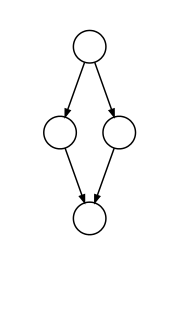
\includegraphics[width=\linewidth]{cfga.png}
		\caption{if-then-else}\label{fig:cfga}		
	\end{subfigure}
	\begin{subfigure}[t]{.24\textwidth}
	\centering
	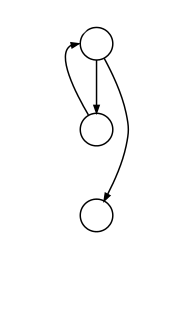
\includegraphics[width=\linewidth]{cfgb.png}
	\caption{while loop}\label{fig:cfgb}		
	\end{subfigure}
	\begin{subfigure}[t]{.24\textwidth}
	\centering
	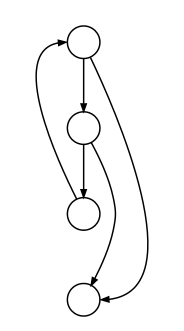
\includegraphics[width=\linewidth]{cfgc.png}
	\caption{natural loop with two exit points}\label{fig:cfgc}		
	\end{subfigure}
	\begin{subfigure}[t]{.24\textwidth}
	\centering
	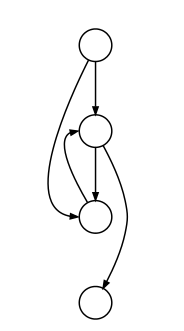
\includegraphics[width=\linewidth]{cfgd.png}
	\caption{loop with two entry point}\label{fig:cfgd}		
	\end{subfigure}

	\caption{Control Flow Graph of different statements and loops}\label{fig:cfg}
\end{figure}

\subsection{Cyclomatic Complexity}
Cyclomatic complexity is a software metric to determine the complexity of a single function, a module, a method, some classes, or the entire program.

It is measured starting from a Control Flow Graph of the program and indicates the number of linearly independent paths of it. 
\\
The formula to calculate the complexity is:

\texttt{M =  E - N + 2P},\\
where \texttt{E} indicates the number of \textit{edges}, \texttt{N} specifies the number of \textit{nodes}, and \texttt{P} indicates the number of \textit{connected components}.\\

If the entry point and exit point are connected, we have a strongly connected graph, and the formula for complexity is slightly different: 

\texttt{M = E - N + P}

\begin{algorithm}
	\caption{Example of function with different loops and statements}\label{alg:complexity}
	\begin{algorithmic}[1]
		
		\setcounter{ALG@line}{0}
		\While{not \texttt{EOF}}
		\State{\texttt{Read} $record$}
		\setcounter{ALG@line}{1}
		\If{$field1 = 0$}
		\State{$total \gets total + field1$}
		\setcounter{ALG@line}{2}
		\State{$counter \gets counter + 1$}
		\Else{ }
		\setcounter{ALG@line}{3}
		\If{$field2 = 0$}
		\State{\texttt{Print} $counter$, $total$}
		\setcounter{ALG@line}{4}
		\State{$counter \gets 0$}
		\Else{}
		\setcounter{ALG@line}{5}
		\State{$total \gets total - field2$}
		
		\EndIf
		\State{\textbf{end if}}
		
		\EndIf
		\State{\textbf{end if}}
		\setcounter{ALG@line}{7}
		\State{\texttt{Print} \textit{End record}}
		
		
		
		\EndWhile
		
		\State{\texttt{Print} $counter$}
		
		
		\setcounter{ALG@line}{0}
		
		
	\end{algorithmic}
\end{algorithm}

Algorithm \ref{alg:complexity} shows an example of function with different loops and statements,which corresponding Control Flow Graph is given in Figure \ref{fig:complexity_ex}. The numbers before the lines represent the id of the basic block to which they belong, i.e. the graph's nodes.

Being \textbf{node \#1} the entry node, and \textbf{node \#9} the exit code, we can manually calculate the number of independent path of the function:
\begin{itemize}
	\item 1, 9
	\item 1, 2, 3, 8, 1, 9
	\item 1, 2, 4, 5, 7, 8, 1, 9
	\item 1, 2, 4, 6, 7, 8, 1, 9
\end{itemize}

	Using the formula presented above, it is possible to calculate the complexity of the function that is equal to 4. $M = 11 - 9 + 2 \times 1 = 4$, where 11 is the \textit{number of edges}, 9 the \textit{number of nodes}, and $2 \times 1$ the \textit{number of connected components}. The complexity calculated equals the number of independent paths of the graph.

\begin{figure}[!h]
	\centering
	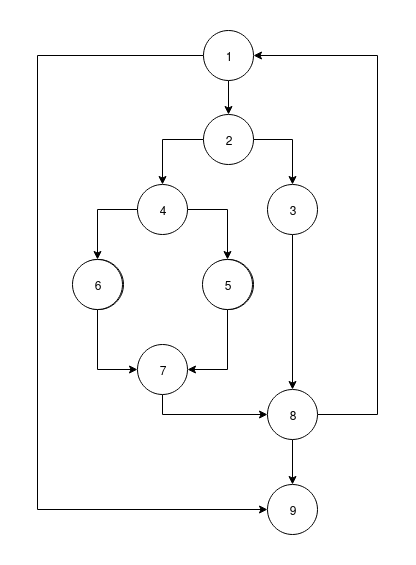
\includegraphics[width=0.6\columnwidth]{complexity.png}
	\caption{Control Flow Graph of Algorithm \ref{alg:complexity}}
	\label{fig:complexity_ex}
\end{figure}


\section{Reverse Engineering tools}

There are a lot of tools in the market that helps in reverse engineering. Some of them have tons of functionalities, and others can do just a few things.

The most important is \textbf{IDA}, a reverse engineering software developed by Hex-Rey that can achieve different things. It is available in a free version and a pro version. 

It is compatible with most of the executable from different OSes, such as \texttt{PE}, \texttt{ELF}, \texttt{Mach-O}, or even raw binaries. It has extensive support and compatibility with almost every family processors.

The free version contains all the features necessary for some basic reverse engineering; it has a disassembler and performs an automatic analysis of the sample, determining the API used, which parameters are passed to them, and other information. 

The analyst can navigate the code and add some notation, rename functions, and variables, to better understand the behavior of the binary. However, most of the functionalities works only with the PRO version, which costs 9000\$.

The main features of IDA PRO \cite{ida} are the debugger that lets the analyst debug the executables, the possibility of writing scripts to run against the sample, and a disassembler to revert the binary into some source code. 


Another famous framework for RE is \textbf{radare2} \cite{radare2}. It is free and offers a decompiler and a disassembler.  It is compatible with tons of processors, and executable types. It comes with a set of command-line utilities that can be used individually or together, but it also has a graphic interface to navigate the code and the possibility of running scripts. However, it is not user-friendly as other tools .

\textbf{Ghidra} \cite{ghidra} is a novel open-source reverse engineering framework developed by the National Security Agency (\textbf{NSA}). It facilitates the analysis of malicious code and malware like viruses and can give cybersecurity professionalists a better understanding of potential vulnerabilities in their networks and systems. It is a direct competitor of IDA PRO because it offers almost all the features that IDA PRO has, but Ghidra is entirely free. It is possible to run a headless version of Ghidra, and control it by remote. We installed it on a virtual machine on a server and use it to run headless scripts on the executables to extract information about the binaries.

We chose to run our tests on \textbf{Ghidra} for different reasons. First of all, it is entirely free and open-source.
Secondly, it has an headless version of the framework. The possibility of a headless version was perfect for our needs because we can let it run on a server, always powered on, without bothering about resource consumption. 
Moreover, we wanted to simplify as much as possible the extraction of features, and we do not want merging results from different tools, so we decided to use only one software. 
Last but not least, the scripting part of Ghidra was perfect for running analysis and extracting information from the samples. 

The only inconvenient is that, since it was released less than a year ago, the documentation, the support, and the community are not well developed, so at first was hard understanding how the software works.
\section{Ghidra}

This section covers the Ghidra's features regarding the disassembled code, decompiler, Control Flow Graph and complexity presented above.
 
\begin{figure}[ht!]
	\centering
	
\includegraphics[width=0.35\textwidth]{ghidra}
	
\end{figure}

\subsection{Disassembled code}

The extraction of disassembled code is an easy and fast task. Ghidra's documentation provides all the information on how to correctly use the disassembler. 

Ghidra does not have a functionality to extract all the disassembled code, like in the GUI. But it is possible, for each function, to iterate the instructions in a given address space range. The instruction object has a \texttt{toString()} method that returns the disassembled line, that we use to create the features needed.

\subsection{PCode}
PCode is a register transfer language developed by NSA for the reverse engineering framework Ghidra. The idea behind PCode is to create a language as general as possible, to let it adapt to as many different processors architecture. An intermediate language that can model the behavior of different processors is fundamental to develop a comprehensive reverse engineering framework.

The idea behind PCode is that each processor instruction can be expressed as a sequence of PCode. Developers translated each instruction into a sequence of PCode operation as input and output variables (\textbf{varnodes}).

The entire set of single PCode instruction comprises a set of arithmetic and logic instructions that almost all processors perform. The direct translation of the instructions into those operations is called raw-PCode, which can be used to emulate a single processor instruction directly. NSA developed the PCodes to facilitate the construction and the analysis of a data flow graph of disassembled instructions.

A PCode operation is the analog of a machine instruction.  All PCode operations have the same format; they have one or mode varnode as input, and optionally they can have an output. Only the output varnode can be modified. 

\subsubsection{Address Space}

The address space for p-code is a generalization of RAM. It represents an indexed sequence of bytes in memory that PCode can read and write into it. The address space has an identifying name, a size indicating the number of distinct indexes of memory, and an endianness that specify the encoding used to store integers and multi-byte values into the space address.

A regular processor has a RAM space to model memory accessible via its data bus, a register space to model the processor's registers, and usually a constant space to store all the constants used by PCodes. All the data that PCode handles must be stored into an address space. 
PCode generally uses a temporary address space to store intermediate values when modeling the processor's instructions. 
The implementation of a processor can have as many address spaces as it needs.


\subsubsection{Varnode}
A varnode is a generalization of a register or memory location and has the functionality of handle the data manipulated by PCodes. It is composed of an address space, an offset into the address space, and a size. 
A varnode is a sequence of contiguous bytes that can be treated as a single value. The address and the size identify the varnode. Even if they have no type, some PCode operations can cast them into three types: integer, boolean, or floating-point. 

In the case of integer values, the PCode operation represents the varnode using the endianness linked with the address space.
In the case of floating-point, the operation uses the encoding of the varnodes that depends on its size.
In the case of boolean values, the varnode has a single byte that can be 0 for false, 1 for true.

If the varnode's address space is in the constant space, the varnode is a constant or an immediate value. In this case the size of the varnode is the size or the precision available for the encoding of the constant.



\subsection{Control Flow Graph}
\label{subsec:cfg_ghidra}
We rely on Ghidra's PCode representation to build our dataset for \textit{Control Flow Graph}. Ghidra contains three different scripts for analyzing the flow of a program, and we studied those scripts to understand how Ghidra manages the PCode and their flow. The script iterates all the functions of the given sample and generates a .json file with the extracted data.

Ghidra offers a \texttt{DecompileInterface}, a class that can decompile a function, and that returns an  \texttt{DecompiledResult} object with all the information needed. It is also possible to set different options to the \texttt{DecompileInterface} using the \texttt{DecompileOption} class. The resulting object contains an instance of \texttt{HighFunction}, a high-level abstraction associated with a low-level function made up of assembly instructions. The \texttt{HighFunction} object offers the possibility to iterate over the BasicBlocks of the corresponding function so we can analyze all the blocks and create our graph.

We save the information gathered into a \texttt{.json} file with the following structure:
The \texttt{.json} is composed of an array of basic blocks, each of which has an index, a list of PCodes, and two lists, one containing the indexes of the previous basic blocks and the other one the indexes where the basic block points, i.e., the flow of our function. The PCodes have a field with the associated PCode operation, a list of input varnodes, and a possible output varnode.

The main problem encountered running the script is the decompilation time. Some functions are intricate, and when they come to decompile, Ghidra can take a very long time, even 25 minutes per sample.  Furthermore, the \texttt{DecompileOption} has a field indicating the maximum dimension of the payload of the decompiled function. The default value is 50MB, but for some specific functions, it is still low, and we need to increase it to 500MB to correctly decompile all the functions.

\subsection{Cyclomatic Complexity}


Ghidra offers a class to compute the complexity of a function, \texttt{CyclomaticComplexity}. This class has a method to calculate the cyclomatic complexity of a function by decomposing it into a flow graph using a \texttt{BasicBlockModel}. During the decompilation, we calculate the complexity of each function and stores it into the .json file.


\section{Scikit-learn}
Scikit-learn \cite{scikit-learn} is a Python module integrating a wide range of state-of-the-art machine learning algorithms for medium-scale supervised and unsupervised problems. 

It is open-source, commercially usable, and contains many modern machine learning algorithms for classification, regression, clustering, feature extraction, and optimization. For this reason, Scikit-learn is often the first tool in a Data Scientists toolkit for machine learning of incoming data sets. 

Scikit-learn depends on \textit{NumPy} and \textit{pandas} modules.\textit{NumPy} (Numerical Python) \cite{numpypandas} is an open-source module for Python designed for mathematical and scientific computation on multi-dimensional arrays. It provides various functions for computations on arrays and matrices.
\textit{Pandas} \cite{numpypandas} is an open-source module for Python too. It is similar to \textit{NumPy}, and provides high-performance structures,called DataFrame, and different data analysis tools. A DataFrame is a 2d table similar to a spreadsheet, it has rows names and columns labels, and provides additional functionalities like plotting graph.

We choose Scikit-learn as a machine learning library because it is the most used in literature, and it has a great community and support. Moreover, it offers all the models and methods required by our work. 
\section{Jupyter Notebook}

The Jupyter Notebook  \cite{jupyter} is an open-source web application that allows you to create and share documents that contain live code, equations, visualizations and narrative text. Uses include: data cleaning and transformation, numerical simulation, statistical modeling, data visualization, machine learning, and much more.

We choose Jupyter because it excellently fits our need for remote running. In the same server, where we installed Ghidra, we installed Jupyter, and we enabled it to run remotely, with the proper precautions. This setup allows us to remotely work without any problem. 

Machine learning tasks are often time and computationally expensive, so running them on a personal computer would be slower due to limited computer resources, and it would keep the workstation busy.
